 % The main file for CAMP reports
 % Don't put any content in here. 
 % Don't even include content files by using \input or \inlcude. 
 % Put your content to TEXT.TEX or include it there using \input.
 % Uses:
 %		SETTINGS.TEX	contains the settings for this document
 %		COMMANDS.TEX	contains commands which can be used while writing
 %		INFO.TEX			contains the author, title and so on for the cover
 %		COVER.TEX			formats the front cover of the document
 %		ABSTRACT.TEX	contains the abstract to be included (if needed)
 %		TEXT.TEX			contains the actual content of the document
 %		BIB.BIB				containt the BibTeX entries for the document
 
 
%% Draft document mode
%% Final document
\documentclass[11pt,a4paper,bibtotoc,idxtotoc,headsepline,footsepline,footexclude,BCOR12mm,DIV13]{scrbook}

%\documentclass[11pt,a4paper,bibtotoc,idxtotoc,headsepline,footsepline,footexclude,BCOR20mm,DIV10]{scrbook}

% KOMA-Optionen:
%  bibtotoc: include bibliography in table of contents
%  idxtotoc: include index in table of contents
%  headsepline: use horizontalline under heading
%  BCOR: binding correcion (Bindungskorrektur) (e.g.: BCOR5mm)
%  DIV: Number of sheet sections (used for layout) (e.g.: DIV12) 



% include title and author information for the cover
% Set here the title, authors and other stuff to be used for the cover
% This file is used by MAIN.TEX

% set title, authors and stuff for the cover
\def\doctype{Diplomarbeit in Informatik}
\def\title{Applications of Deep Learning in Natural Language Processing in \\
German for Document Classification and Information Extraction }
\def\titleGer{Die grosse Arbeit}
\def\author{Miguel Fernando Cabrera Granados}
\def\date{March 15, 2014}

% text to appear in the footer
\def\footertext{}


% include settings
% Included by MAIN.TEX
% Defines the settings for the CAMP report document

\renewcommand{\sectfont}{\normalfont \bfseries}        % Schriftart der Kopfzeile

% manipulate footer
\usepackage{scrpage2}
\pagestyle{scrheadings}
\ifoot[\footertext]{\footertext} % \footertext set in INFO.TEX
%\setkomafont{pagehead}{\normalfont\rmfamily}
\setkomafont{pagenumber}{\normalfont\rmfamily}

%% allow sophisticated control structures
\usepackage{ifthen}

% use Palatino as default font
\usepackage{palatino}

% enable special PostScript fonts
\usepackage{pifont}

% make thumbnails
\usepackage{thumbpdf}

%to use the subfigures
\usepackage{subfigure}


\usepackage{colortbl}

\usepackage{acronym}


%% show program code\ldots
%\usepackage{verbatim}
%\usepackage{program}

%% enable TUM symbols on title page
\usepackage{styles/tumlogo}


\usepackage{multirow}

%% use colors
\usepackage{color}

%% make fancy math
\usepackage{amsmath}
\usepackage{amsfonts}
\usepackage{amssymb}
\usepackage{textcomp}
\usepackage{yhmath} % f�r die adots 
%% mark text as preliminary
%\usepackage[draft,german,scrtime]{prelim2e}

%% create an index
\usepackage{makeidx}

% for the program environment
\usepackage{float}

%% load german babel package for german abstract
%\usepackage[german,american]{babel}
\usepackage[german,english]{babel}
\selectlanguage{english}
\sloppy

% use german characters as well
\usepackage[latin1]{inputenc}       % allow Latin1 characters

% use initals dropped caps - doesn't work with PDF
\usepackage{dropping}


\usepackage{styles/shortoverview}
%----------------------------------------------------
%      Graphics and Hyperlinks
%----------------------------------------------------

%% check for pdfTeX
\ifx\pdftexversion\undefined
 %% use PostScript graphics
 \usepackage[dvips]{graphicx}
 \DeclareGraphicsExtensions{.eps,.epsi}
 \graphicspath{{figures/}{figures/review}} 
 %% allow rotations
 \usepackage{rotating}
 %% mark pages as draft copies
 %\usepackage[english,all,light]{draftcopy}
 %% use hypertex version of hyperref
 %\usepackage[hypertex,hyperindex=false,colorlinks=true,hidelinks]{hyperref}
\else %% reduce output size \pdfcompresslevel=9
 %% declare pdfinfo
 %\pdfinfo { 
 %  /Title (my title) 
 %  /Creator (pdfLaTeX) 
 %  /Author (my name) 
 %  /Subject (my subject	) 
 %  /Keywords (my keywords)
 %}
 %% use pdf or jpg graphics
 \usepackage[pdftex]{graphicx}
 \DeclareGraphicsExtensions{.jpg,.JPG,.png,.pdf,.eps}
 \graphicspath{{figures/}} 
 
 %% Load float package, for enabling floating extensions
 \usepackage{float}
 
 %% allow rotations
 \usepackage{rotating}
 %% use pdftex version of hyperref
 \usepackage[pdftex,colorlinks=true,linkcolor=black,hidelinks,citecolor=red,%
 anchorcolor=red,urlcolor=red,bookmarks=true,%
 bookmarksopen=true,bookmarksopenlevel=0,plainpages=false%
 bookmarksnumbered=true,hyperindex=false,pdfstartview=%
 ]{hyperref}

\usepackage{longtable}
%
%\usepackage[pdftex,colorlinks=false,linkcolor=red,citecolor=red,%
% anchorcolor=red,urlcolor=red,bookmarks=true,%
% bookmarksopen=true,bookmarksopenlevel=0,plainpages=false%
% bookmarksnumbered=true,hyperindex=false,pdfstartview=%
% ]{hyperref}
\fi




%% Fancy chapters
%\usepackage[Lenny]{fncychap}
%\usepackage[Glenn]{fncychap}
%\usepackage[Bjarne]{fncychap}

%\usepackage[avantgarde]{quotchap}

% set the bibliography style
%\bibliographystyle{styles/bauermaNum}
%\bibliographystyle{alpha}
\bibliographystyle{plain}


% include commands
% Commands to be used within the TUM report document
% Included by MAIN.TEX
% Please include your own cool commands here. 
% Be only sure to comment it sufficiently so others can use it.

%-------------------------------------------------------------
%                      Own Commands
%-------------------------------------------------------------


%-------------------------------------------------------------
% math stuff -------------------------------------------------

% nice R, N, C
\newcommand{\nat}{\mathbb{N}}
\newcommand{\real}{\mathbb{R}}
\newcommand{\compl}{\mathbb{C}}



% norm
\newcommand{\norm}[1]{\left\| #1 \right\|}

% un demi
\newcommand{\half}{\frac{1}{2}}

% parantheses
\newcommand{\parenth}[1]{ \left( #1 \right) }
\newcommand{\bracket}[1]{ \left[ #1 \right] }
\newcommand{\accolade}[1]{ \left\{ #1 \right\} }
%\newcommand{\angle}[1]{ \left\langle  #1 \right\rangle }

% partial derivative: %#1 function, #2 which variable
% simple / single line version
\newcommand{\pardevS}[2]{ \delta_{#1} f(#2) }
% fraction version
\newcommand{\pardevF}[2]{ \frac{\partial #1}{\partial #2} }

% render vectors: 3 and 4 dimensional
\newcommand{\veciii}[3]{\left[ \begin{array}[h]{c} #1 \\ #2 \\ #3	\end{array} \right]}
\newcommand{\veciv}[4]{\left[ \begin{array}[h]{c} #1 \\ #2 \\ #3 \\ #4	\end{array} \right]}

% render matrices: 3  dimensional (arguments in row first order)
\newcommand{\matiii}[9]{\left[ \begin{array}[h]{ccc} #1 & #2 & #3 \\ #4 & #5 & #6 \\ #7 & #8 & #9	\end{array} \right]}
%DOESN'T WORK,DON'T KNOW WHY \newcommand{\mativ}[16]{\left[ \begin{array}[h]{cccc} #1 & #2 & #3 & #4 \\ #5 & #6 & #7 & #8 \\ #9 & #10 & #11 & #12 \\ #13 & #14 & #15 & #16 \end{array} \right]}


%-------------------------------------------------------------
%-------------------------------------------------------------


%-------------------------------------------------------------
% some abreviations ------------------------------------------
\newcommand{\Reg}{$^{\textregistered}$}
\newcommand{\reg}{$^{\textregistered}$ }
\newcommand{\Tm}{\texttrademark}
\newcommand{\tm}{\texttrademark~}
\newcommand {\bsl} {$\backslash$}

%-------------------------------------------------------------
%-------------------------------------------------------------


%-------------------------------------------------------------
% formating --------------------------------------------------

% Theorem & Co environments and counters
\newtheorem{theorem}{Theorem}[chapter]
\newtheorem{lemma}[theorem]{Lemma}
\newtheorem{corollary}[theorem]{Corollary}
\newtheorem{remark}[theorem]{Remark}
\newtheorem{definition}[theorem]{Definition}
\newtheorem{equat}[theorem]{Equation}
\newtheorem{example}[theorem]{Example}
\newtheorem{algorithm}[theorem]{Algorithm}

% inserting figures
\newcommand{\insertfigure}[4]{ % Filename, Caption, Label, Width percent of textwidth
	\begin{figure}[htbp]
		\begin{center}
			\includegraphics[width=#4\textwidth]{#1}
		\end{center}
		\vspace{-0.4cm}
		\caption{#2}
		\label{#3}
	\end{figure}
}




% referecing figures

\newcommand{\refFigure}[1]{ %label
	figure \ref{#1}
}
\newcommand{\refChapter}[1]{ %label
	chapter \ref{#1}
}

\newcommand{\refSection}[1]{ %label
	section \ref{#1}
}

\newcommand{\refParagraph}[1]{ %label
	paragraph \ref{#1}
}

\newcommand{\refEquation}[1]{ %label
	equation \ref{#1}
}

\newcommand{\refTable}[1]{ %label
	table \ref{#1}
}




\newcommand{\rigidTransform}[2]
{
	${}^{#2}\!\mathbf{H}_{#1}$
}

%code, in typewriter
\newcommand{\code}[1]
 {\texttt{#1}}

% comment that appears on the border - very practical !!!
\newcommand{\comment}[1]{\marginpar{\raggedright \noindent \footnotesize {\sl #1} }}

% page clearing
\newcommand{\clearemptydoublepage}{%
  \ifthenelse{\boolean{@twoside}}{\newpage{\pagestyle{empty}\cleardoublepage}}%
  {\clearpage}}


%-------------------------------------------------------------
%-------------------------------------------------------------


\newcommand{\etAl}{\emph{et al.}\mbox{ }}


%\makeindex
	%% inter line spacing
%\linespread{1.0}

\makeglossary

\begin{document}

	\frontmatter
	
	
	% The front cover for the TUM report document.
% Included by MAIN.TEX


%--------------------------------------------------
% The Front Cover
%--------------------------------------------------

% The front cover for the TUM document.
% Included by MAIN.TEX


%--------------------------------------------------
% The Front Cover
%--------------------------------------------------

% correct BCOR - undo at the end !!!
\def\bcorcor{0.15cm}
\addtolength{\hoffset}{\bcorcor}

\thispagestyle{empty}

 \vspace{4cm}
\begin{center}
	       \oTUM{4cm}
	   
	   \vspace{5mm}     
	   \huge FAKULT{\"A}T F{\"U}R INFORMATIK\\ 
	   \vspace{0.5cm}
	 \large DER TECHNISCHEN UNIVERSIT{\"A}T M{\"U}NCHEN\\
    \vspace{1mm}
        
	\end{center}
		

\vspace{15mm}
\begin{center}

   {\Large \doctype}

  \vspace{20mm}
  
  {\huge\bf \title}\\%[3ex]
  
  
  \vspace{15mm}
  
  
  {\LARGE  \author}
  
  \vspace{10mm}
  
  \begin{figure}[h!]
  \centering
   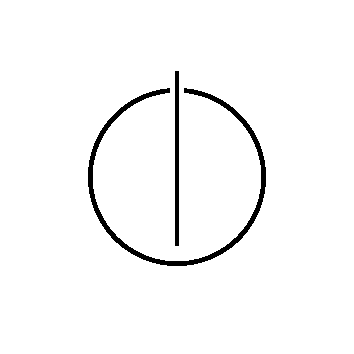
\includegraphics[width=4cm]{styles/informat.png}
  \end{figure}
  
  \end{center}
%	\clearemptydoublepage
%	
%	% The titlepage for the CAMP report document.
% Included by MAIN.TEX


%--------------------------------------------------
% The title page
%--------------------------------------------------

% correct BCOR - undo at the end !!!
\def\bcorcor{0.15cm}
\addtolength{\hoffset}{\bcorcor}

\thispagestyle{empty}

 \vspace{10mm}
\begin{center}
	       \oTUM{4cm}
	   
	   \vspace{5mm}     
	   \huge FAKULT{\"A}T F{\"U}R INFORMATIK\\ 
	   \vspace{0.5cm}
	 \large DER TECHNISCHEN UNIVERSIT{\"A}T M{\"U}NCHEN\\
        
	\end{center}
		

\vspace{10mm}
\begin{center}

   {\Large \doctype}

  \vspace{10mm}
  
  {\LARGE \title}\\
  
  
  \vspace{10mm}
  
  
  {\LARGE  \titleGer}\\
  
  
  \vspace{10mm}

    %\hfill
    \begin{tabular}{ll}
	   \Large Author:     & \Large \author  \\[2mm]
	   \Large Supervisor:    & \Large Prof. Dr. However Wasit \\[2mm]				
	   \Large Advisor:	& \Large Dipl.Inf. Whoever Didit\\[2mm]
	   \Large Date:       & \Large August 15, 2006
	 \end{tabular}
	 
	 \vspace{5mm}
	 
	 \begin{figure}[h!]
  \centering
   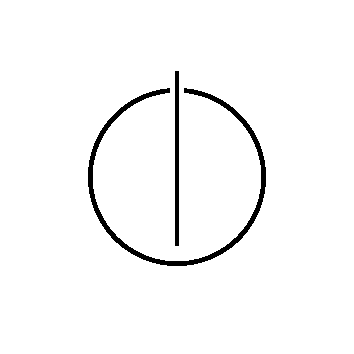
\includegraphics[width=4cm]{styles/informat.png}
  \end{figure}
   

\end{center}

% undo BCOR correction
\addtolength{\hoffset}{\bcorcor}

	
	
%	\input{components/cover_maschmeyer}
	\clearemptydoublepage
	
	% The titlepage for the CAMP report document.
% Included by MAIN.TEX


%--------------------------------------------------
% The title page
%--------------------------------------------------

% correct BCOR - undo at the end !!!
\def\bcorcor{0.15cm}
\addtolength{\hoffset}{\bcorcor}

\thispagestyle{empty}

 \vspace{10mm}
\begin{center}
	       \oTUM{4cm}
	   
	   \vspace{5mm}     
	   \huge FAKULT{\"A}T F{\"U}R INFORMATIK\\ 
	   \vspace{0.5cm}
	 \large DER TECHNISCHEN UNIVERSIT{\"A}T M{\"U}NCHEN\\
        
	\end{center}
		

\vspace{10mm}
\begin{center}

   {\Large \doctype}

  \vspace{10mm}
  
  {\LARGE \title}\\
  
  
  \vspace{10mm}
  
  
  {\LARGE  \titleGer}\\
  
  
  \vspace{10mm}

    %\hfill
    \begin{tabular}{ll}
	   \Large Author:     & \Large \author  \\[2mm]
	   \Large Supervisor:    & \Large Prof. Dr. However Wasit \\[2mm]				
	   \Large Advisor:	& \Large Dipl.Inf. Whoever Didit\\[2mm]
	   \Large Date:       & \Large August 15, 2006
	 \end{tabular}
	 
	 \vspace{5mm}
	 
	 \begin{figure}[h!]
  \centering
   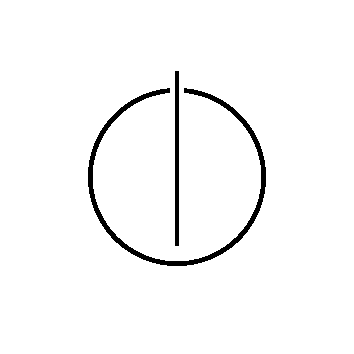
\includegraphics[width=4cm]{styles/informat.png}
  \end{figure}
   

\end{center}

% undo BCOR correction
\addtolength{\hoffset}{\bcorcor}

	
	
	\clearemptydoublepage


\thispagestyle{empty}
\selectlanguage{german}
	\vspace*{0.8\textheight}
	\noindent
	Ich versichere, dass ich diese Diplomarbeit selbst{\"a}ndig verfasst und nur 
	die angegebenen \\Quellen und Hilfsmittel verwendet habe.
	
	\vspace{15mm}
	\noindent
	M{\"u}nchen, den \today \hspace{5cm} \author
\selectlanguage{english}
\newpage
	
	\clearemptydoublepage
\phantomsection
\addcontentsline{toc}{chapter}{Acknowledgements}	


%\chapter*{Acknowledgements}

\vspace*{2cm}

\begin{center}
{\Large \bf Acknowledgments}
\end{center}

\vspace{1cm}




If someone contributed to the thesis... might be good to thank them here.
	
	% Abstract for the TUM report document
% Included by MAIN.TEX


\clearemptydoublepage
\phantomsection
\addcontentsline{toc}{chapter}{Abstract}	





\vspace*{2cm}
\begin{center}
{\Large \bf Abstract}
\end{center}
\vspace{1cm}

The success of machine learning algorithms  depends on the 
representation of the data used.  Specific domain knowledge can be used to
design good representations. However, these representations are limited to a
specific problem  or task, and to the amount of available labeled data.
Another approach is to automatically learn  generic priors that can be used in different
tasks and context. In the field of natural language processing, recent work
has been done in obtaining such priors by learning useful vector representation of
words from unlabeled data. The representations can then be used to improve
existing natural language processing systems.  These word vectors are  obtained using special neural network architectures   
 trained on billions of tokens. However, most of these models  are learned
and evaluated on English language corpora.       In this work,
\textit{Word2vec}, a recent neural network based  toolkit for learning word
representations is used on German language data. The goal is to evaluate the
learned representations of words in different language processing and information
retrieval tasks. In particular, a semantic-syntactic  evaluation set  is
constructed for the German language. In addition to that, the
learned word vector representations are used as features for a classifier of German
language business documents. The learned features outperformed existing handcrafted features and
performed  similar to other state-of-the-art approaches.




%%% Local Variables: 
%%% mode: latex
%%% TeX-master: "../main.tex"
%%% End:



	\tableofcontents
  
  \clearemptydoublepage

\phantomsection
\addcontentsline{toc}{chapter}{Outline of the Thesis}

\begin{center}
	\huge{Outline of the Thesis}
\end{center}




%--------------------------------------------------------------------
\section*{Part I: Introduction and Theory}

\noindent {\scshape Chapter 1: Introduction}  \vspace{1mm}

\noindent  This chapter presents an overview of the thesis and it purpose. Furthermore, it will discuss the sense of life in a very general approach.  \\

\noindent {\scshape Chapter 2: Theory}  \vspace{1mm}

\noindent  No thesis without theory.   \\

%--------------------------------------------------------------------
\section*{Part II: The Real Work}

\noindent {\scshape Chapter 3: Overview}  \vspace{1mm}

\noindent  This chapter presents the requirements for the process.

	\mainmatter
	
	
		% ---------------------------------------------------------------------------
		%
		%Introduction and Background Theory
		%
		% ---------------------------------------------------------------------------
		\part[Introduction and Theory]{Introduction and Theory}
		\label{part:introAndBackgroundTheory}
		\chapter{Introduction}
\label{chapter:Introduction}


From the early days of computers, people have dreamed about machines with intelligence. Computers able to exhibit complex behavior and able to solve tasks assigned by users. If we assume that this problem is too difficult to solve immediately, we can think of several step that will lead towards the development of intelligent machines. One of the first tasks to solve is the one of language understanding, i.e. giving the machine to process and understand human language. This by definition is a hard task even for human beings, as natural language is inherently ambiguous.


Current computational language modeling techniques are based on statistical
measurements and hardcoded rules. Although they perform fairly well in
several tasks, they are far from achieving human like results in many natural
language processing problems. One way to try to achieve human like behavior
in a machine is to emulate the way of human brain works. This is the main
idea behind the initial use of neural networks in the early days of
artificial intelligence in the 60s and 70s. The last decade has seen a
revival of this trend via  \textit{Deep Learning} approaches. \textit{Deep Learning} tries to learn useful high-level representations of data using raw data via hierarchical architectures. This is similar in principle to the theories of brain development proposed by the cognitive neuroscientists in the early 1990s.

In the field of natural language processing, most of the research  has
focused on  trying to obtain words representation that allow to extract
meaning from unlabeled text, mostly in English language.  However,  English
lack of the morphological complexity exhibited by other Germanic and
non-Germanic languages such as German and Spanish. Therefore, it  is of
interest to evaluate what information can extract these models from
morphological richer languages. Besides that, one the performance of these
representation of words is assesed, it is important to design or adapt
machine learning system that can take advantage of these representations.


 % Even if these models have achieved to generate representation containing  interesting relationships among words, there are not still a clear way to use them for improving many existing tasks.


%There are t

% 
%The goal of this thesis is to describe new techniques that have been developed to overcome the simple n-gram models that still %remain basically state-of-the-art today. To prove usefulness of the new approaches, empirical results on several standard data %sets will be extensively described. Finally, approaches and techniques that can possibly lead to automatic language learning %by computers will be discussed, together with a simple plan how this could be achieved.


% current language modeling techniques  are based on 
% - Language understanding via language modelling.
% One way to simiulate this behaviour The Turing test was designed by 

% - Alan Turing and the machine (re-write Mikolov thing)
% - Emulating the using neural computation
% - This important because the implications
% - most of the work has been done in english where other languges exists and their differences 
% - Amount of data of data avaitlable on the web
% - Unlabaled thus impoortant to learn from unlabeled data.
% - Text categorization
% - Better language model will lead us to better understanding of human by the machine.


% From the first day of existence of the computers, people were dreaming about artificial intelligence - machines that would produce complex behaviour to reach goals specified by human users. Possibility of existence of such machines has been controversial, and many philosophical questions were raised - whether the intelligence is not unique only to humans, or only to animals etc. Very influential work of Alan Turing did show that any computable problem can be computed by Universal Turing Machine - thus, assuming that the human mind can be described by some algorithm, Turing Machine is powerful enough to represent it.
% Computers today are Turing-complete, ie. can represent any computable algorithm. Thus, the main problem is how to find configuration of the machine so that it would produce desired behaviour that humans consider intelligent. Assuming that the problem is too difficult to be solved immediately, we can think of several ways that would lead us towards intelligent machines - we can start with a simple machine that can recognize basic shapes and images such as written digits, then scale it towards more complex types of images such as human faces and so on, finally reaching machine that can recognize objects in the real world as well as humans can.
% Other possible way can be to simulate parts of the human brain on the level of indi- vidual brain cells, neurons. Computers today are capable of realistically simulating the real world, as can be seen in modern computer games - thus, it seems logical that with accurate simulation of neurons and more computational power, it should be possible to simulate the whole human brain one day.

\section{Motivation and Objectives}

\label{sec:motivation}

The goal of this thesis is to describe deep learning approaches to learn word features,  performing a empirical study of the performance of such representation in the German language and evaluating the applicability of such methods in existing problems, in particular the field of automated text categorization. 

There are two  main motivations behind this objective. First, it is
interesting to evaluate word representation of languages other than English.
This allows measuring  to some degree the generalization power and the ability to extract useful features of these models. Second,  most of the existing data existing is unlabeled. Thus, developing pipelines that allow to take advantage of large amount of available data  is necessary to improve existing systems that  process natural language.  

For that purpose an empirical evaluation of the \textit{Word2vec} model  on German
language corpora has been chosen. \textit{Word2vec} is a tool that by means of
a neural network learns vector representation of words.
\textit{Word2vec} is used  because it has shown to produce representations
that contain rich relationships among words . In the application area, the
field of automatic document classification of German language document has
been selected. The reason for this is two-fold. On one had, the amount  work
has been done in applying such representation  in the general area of
automated document classification is limited. On the other hand, the nature
of the data set chosen,  from which limited amount of document is available;
offer the perfect chance to evaluate the performance obtained by using
features learned from unlabeled data.

%%- natural language and therefore word vector embeddings model has been mostly evalutated using english as the basic language
% - how these perform on toher languages other than english with more complex grammar and sytax is nonethelss important.

% - word2vec has shown to generate interesting word vector maininigting linear relationships. However, up to this date no applications of these word vector model besides some experiments with translation. 
% - This word explores a previous approach to document classificaion using word word vectors but with two particularities. One the exsitince of an already classifier based on handcrafted features, second the language of work is German, that is a highly inflective language. 


\section{Structure of the Thesis}
\label{sec:structure-thesis}

The theoretical foundation required for the understanding of this thesis is
described in chapter \ref{chap:related_work}. This chapter also gives an
overview about related work in the of language modeling and text
representations.  In particular, it describes the model that led to the
development of \textit{Word2vec}.
 Chapter \ref{chap:word2vec_description} describes in detail the architecture
 \textit{Word2vec}. Afterwards in  chapter \ref{chapter:wor2vec_german}  
 an empirical evaluation of the \textit{Word2vec} model on a German language
 corpus is performed.  Chapter \ref{chap:rel_word2vec_doc_classification} explores the
 application of these representations in the field automated text
 categorization. Finally, in chapter \ref{chap:conclusion_future_work} the
 thesis is concluded and possible future work is outlined.

% 4 guide through the development process of the WAF. Chapter 5 discusses an evaluation of different wifi AP localization techniques. Finally, in chapter 6 the thesis is concluded and an outlook for future work is given.


% \section{Claims of the Thesis}
% \label{sec:claims-of-the-thesis}



 



%%% Local Variables: 
%%% mode: latex
%%% TeX-master: "../main.tex"
%%% End:

		
		
		%
		%% ---------------------------------------------------------------------------
		%%
		%% Fully Automated Calibration for Ultrasound
		%%
		%%% ---------------------------------------------------------------------------
		\part[The 2nd Part]{The Second Part}
		\label{part:secondP}
		
		
		% ---------------------------------------------------------------------------
		%
		% Appendix
		%
		% ---------------------------------------------------------------------------
		
		\part*{Appendix}
		\addcontentsline{toc}{part}{Appendix}
		
		\appendix %---------------------------------------
		
		\chapter{Detailed Descriptions}
%\section{Detailed Validation Results}
\label{chapter:DetailedDescriptions}
Here come the details that are not supposed to be in the regular text.
		
	


  \clearemptydoublepage
  
	\bibliography{bibliography/literature}
	
 
\end{document}

